\chapter{引言}
在本章中,我们介绍信息论与编码理论的基本情况,使大家对信息理论和编码理论的全貌有一个大致的了解.

\begin{introduction}
 \item 信息论的早期酝酿
 \item Shannon信息论的建立与发展
 \item 信息论的近期发展
 \item 信息的度量问题
 \item 通信系统的基本要素与模型
 \item 通信系统的概率统计模型
\end{introduction}
\section{信息论的形成与发展}

\textbf{一、信息论的早期酝酿}

1.早期编码问题

在有线和无线电通信产生的同时,编码技术随之产生,早期的编码有Morse码和Bodo码.他们将文字通过点、划、空等信号给以表达,这些码虽然很原始,但它们实现了从文字到通讯信号的转变.中文通信等用的是电报码的方式,先将汉字转成数字,再用电码发射.

2.通信的有效性和可靠性

随着通信距离的加大,出现了信号强度衰减与噪声干扰的问题, 因此, 如何克服噪声千扰问题就成为通信技术中的一个迫切问题.为解决这些问题, 人们对通信中的各种因素进行分析, 发现在通信技术中,通信的数量与质量存在相互制约的关系.如果牺牲通信的数量, 则可以达到提高质量的目的, 但二者之间究竟有何定量关系,却无法说明.到了20世纪20 年代,奈奎斯特等人对上述问题进行了一系列讨论, 说明了信息传递的速率与带宽成正比,信息的度量与信号的概率分布、对数函数有关等等.

\textbf{二、Shannon信息论的建立与发展}

信息论的产生以1948年C.E.Shannon发表的 “通信的数学理论” 这一奠定性论文为起始,作为信息理论的奠基人,对其主要生平作一个简单的介绍.

Claude Edwoods Shannon(香农、仙农)  

C.E.Shannon(1916-2001) 数学家, 工程学家.信息论创始人,奠基人,电子计算机理论的重要奠基人之一.代表性著作:\\
(1)1938年(22岁),发表著名论文《继电器和开关电路的符号分析》文中首次使用了比特(bit)的概念.\\
(2) 1948年, 《通信的数字理论》第一次提出信息量的概念,并且应用数理统计的方法来研究通信系统, 从而创立了影响深远的信息论.\\
(3)1949年, 《噪声下的通信》经典的阐明了通信的基本问题, 提出了通信系统的模型, 给出了信息量的数字表达式, 解决了通道容量, 信源统计特性, 信源编码, 信道编码等有关精确地传递通信符号的基本技术问题.\\
(4)1956年, 《噪声信道的零差错容量》开拓了零差错容量的研究领域.\\
(5)1959年, 《在保真度准则下的离散信源编码定理》推动了信息率失真理论研究等.

Shannon提出完善信息理论离不开对编码问题的研究, 因此信息论与编码理论密不可分.

1.Shannon信息论的确立期(1948年-20世纪60年代)
此阶段主要是对Shannon理论进行研究与说明, 包括对通信系统的数学模型和基本问题的说明与讨论.

2.Shannon信息论的发展期(20世纪70-80年代)这一时期主要内容在 “率失真理论”与 “多用户信息论” 方面,后发展为数据压缩理论.

\textbf{三、信息论的近期发展}

信息论近期发展的主要特点是向多学科结合方向发展.

1. 信息论与密码学(通信编码问题的一种表现形式)

2. 算法信息论与分形数学 (信息论, 计算机科学, 分形理论的共同本质,决定如何互相等价转化).

3.信息论在统计与智能计算中的应用\\
(1) 智能计算中的信息统计问题.\\
(2)信息计算与组合投资决策关系密切.\\
(3)编码理论在与试验设计, 假设检验理论的结合中发挥了重要作用.

4.信息论在工程领域中的应用

主要是编码理论在工程领域有广泛应用.


\section{信息与编码理论的主要内容}

\textbf{一、信息的度量问题}

Shannon熵是Shannon信息论中信息的度量基础,它与概率分布有关,以不肯定性(不确定性)作为度量信息的基础,即信息量是描述消息中不确定性的概念.
例如:一个消息 “太阳从东边升起,西边落下”,这一消息中没有任何信息, 即含有的信息量为 0 .这是一确定的消息, 不含有任何的不肯定性(不确定性).


\textbf{二、通信系统的基本要素与模型}

1. 一个系统由以下基本要素与模型\\
(1)信源:产生信息的来源,信源产生的信息称为消息.\\
(2)信道:传递信息的通道,消息通过信道以信号的形式传播.\\
(3)编码:由消息产生信号的运算.\\
(4)译码:由信号还原为消息的运算称为译码.\\
(5)通信系统: 由信源、信道、编码和译码四个要素组成.\\
(6) 用户:通信系统的使用者,分为发送者和接收者.

2.通信系统的基本模型
\begin{figure}[ht]
    \centering
    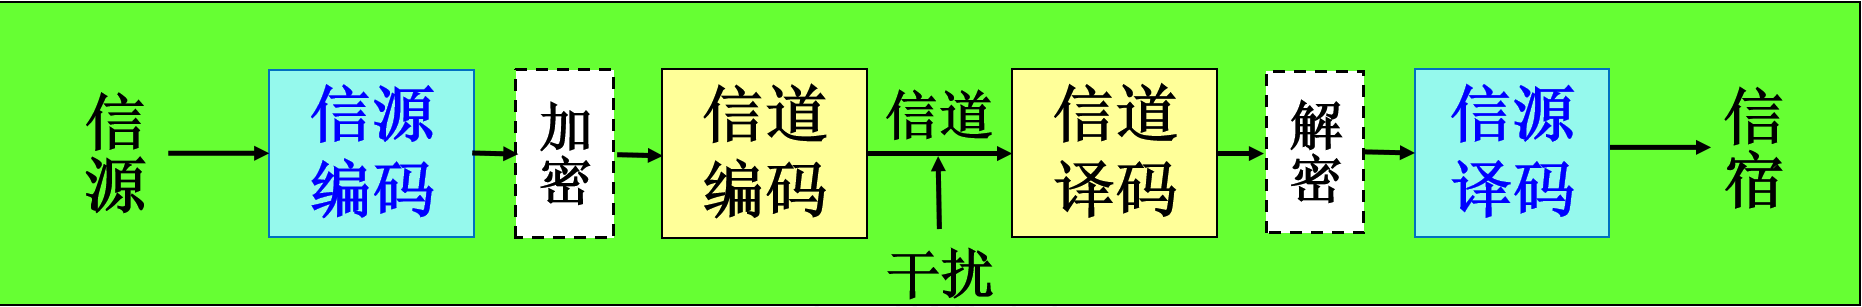
\includegraphics[width=0.5\linewidth]{image/0.png}
\end{figure}
由于干扰的存在, 信道的输出信号可能与输入信号不同, 从而使得还原消息与原始消息可能不同,这种现象称为通信误差,是通信系统中需要克服的现象.

克服通信误差 $ \left\{\begin{array}{l}\text { 硬件途径: 元器件改进, 降低噪声干扰 } \\ \text { 软件途径: 用编码方式克服 } \rightarrow \text { 纠错和检错码 }\end{array}\right. $


\textbf{三、通信系统的概率统计模型}

1. 信源的概率统计模型

\begin{definition}
    信源是消息的来源, 用 $ \mathscr{S}=[\mathscr{X}, p(x)] $ 来表示, 其中 $ \mathscr{X} $ 为信源字母表, 是消息中可能使用的全体符号, 它的元素 $ x \in \mathscr{X} $ 是信源字母表中的字母, $ p(x) $ 是字母 $ x $ 的使用概率.由概率分布的性质知, 对 $ \forall x \in \mathscr{X} $, 有 $ p(x) \geqslant 0 $,且 $ \sum\limits_{x \in \mathscr{X}} p(x)=1 $ .
\end{definition}


2. 信道的概率统计模型

信道由以下因素组成:输入信号字母集,输出信号字母集与转移概率分布, 分别记为\\ $ \{\mathscr{U}, \mathscr{V}, p(v \mid u), u \in \mathscr{U}, v \in \mathscr{V}\} $, 其中 $ \mathscr{U} $ 为全体能使用的输入信号字母集,简称为输入信号字母表, $ \mathscr{V} $ 是可能输出的信号字母集,简称为输出信号字母表.若 $ u \in \mathscr{U}, v \in \mathscr{V} $, 表示输入和输出信号字母, 而 $ p(v \mid u) $ 是输入、输出信号字母的转移概率, 即当输入信号为 $ u $, 输出信号为 $ v $ 的概率, 有 $ p(v \mid u) \geqslant 0, \sum\limits_{v \in \mathscr{V}} p(v \mid u)=1 $ .

\begin{definition}
    信道的概率统计模型为 $ \mathscr{C}=(\mathscr{U}, p(v \mid u), \mathscr{V}) $, 其中 $ \mathscr{U}, \mathscr{V} $ 分别是输入和输出信号字母表, $ p(v \mid u) $ 是输入和输出信号字母的转移概率.
\end{definition}



3. 编码与译码的函数表示
\begin{definition}
    由消息变为信道输入信号的运算称为编码,由信道输出信号变为还原消息的运算称为译码.记 $ \mathscr{Y} $ 为还原消息字母表.则 $ f: \mathscr{X} \rightarrow \mathscr{U}, g: \mathscr{V} \rightarrow \mathscr{Y} $ 分别是编码和译码运算, 在通信系统中,一般 $ \mathscr{U} $ 与 $ \mathscr{V} $ 相同,但也可以不同.
\end{definition}

4. 通信系统的数学模型
\begin{definition}
    称信源与信道的组合为通信系统, 记为
$$
\mathscr{E}=\{\mathscr{S}, \mathscr{C}\}=\{\mathscr{X}, p(x), \mathscr{U}, p(v \mid u), \mathscr{V}\}
$$
对于一个通信系统 $ \varepsilon $, 如果编码和译码函数 $ f, g $ 给定, 那么我们称这个通信系统是有编码的通信系统,记为
$$
\mathscr{E}(f, g)=\{\mathscr{S}, \mathscr{C},(f, g), \mathscr{Y}\}=\{\mathscr{X}, p(x), \mathscr{U}, p(v \mid u), \mathscr{V},(f, g), \mathscr{Y}\}
$$
\end{definition}


5. 由通信系统决定的随机变量

因为通信系统由一系列概率分布组成,因此我们可以用随机变量表示, 记:\\
$ \bar{\xi} $ 由信源 $ \mathscr{S}=\{\mathscr{X}, p(x)\} $ 决定的随机变量.\\
$ \xi $ 由信道输入信号决定的随机变量.\\
$ \eta $ 由信道输出信号决定的随机变量.\\
$ \bar{\eta} $ 由还原消息决定的随机变量.\\
$ \bar{\xi} $ 在 $ \mathscr{X} $ 上取值, 其概率分布为 $ p(x) $ .

\begin{theorem}
    如果有编码的通信系统 $ \mathscr{E}(f, g) $ 给定, 则这个通信系统的随机变量 $ (\bar{\xi}, \xi, \eta, \bar{\eta}) $ 的联合概率分布确定, 它们的联合概率分布 $ p(x, u, v, y)=p(x) f(u \mid x) p(v \mid u) g(y \mid v) $ ,其中 $ p(x), p(v \mid u) $ 分别由信源 $ S $ 和信道 $ C $ 给定.
$$
f(u \mid x)=\left\{\begin{array}{ll}
1, & u=f(x) \\
0, & u \neq f(x)
\end{array}\right.
$$
$$
g(y \mid v)=\left\{\begin{array}{ll}
1, & y=g(v) \\
0, & y \neq g(v)
\end{array}\right.
$$
这时, $ (\bar{\xi}, \xi, \eta, \bar{\eta}) $ 构成一个马尔可夫(Markov)链,因为当 $ \xi $ 固定时, $ \bar{\xi} $ 与相互独立,而当 $ \eta $ 固定时, $ (\bar{\xi}, \xi) $ 与 $ \bar{\eta} $ 相互独立.
\end{theorem}

有关概率记号: $ p(x, u, v, y)=P_{r}\{(\bar{\xi}, \xi, \eta, \bar{\eta})=(x, u, v, y)\} $
$$
\begin{array}{l}
p(x)=\operatorname{Pr}\{\bar{\xi}=x\} \\
p(v \mid u)=\operatorname{P} r\{\eta=v \mid \xi=u\}
\end{array}
$$
其中, $ P_{r}(A) $ 表示事件 $ A $ 发生的概率, $ P_{r}(A \mid B) $ 表示事件 $ A $ 关于事件 $ B $ 的条件概率.
$$
P(A)=P_{r}(A) \quad P(A \mid B)=P_{r}(A \mid B)
$$

\begin{definition}
    如果随机变量 $ (\bar{\xi}, \xi, \eta, \bar{\eta}) $ 的概率分布为 $ p(x, u, v, y)=p(x) f(u \mid x) p(v \mid u) g(y \mid \underline{v}) $, 则称 $ (\bar{\xi}, \xi, \eta, \bar{\eta}) $ 是由通信系统 $ \mathscr{E}(f, g) $ 决定的随机变量, 如果 $ (\bar{\xi}, \xi, \eta, \bar{\eta}) $ 构成一个马尔可夫链, 那么记之为:
$$
\bar{\xi} \longrightarrow \xi \longrightarrow \eta \longrightarrow \bar{\eta}
$$
\end{definition}

\section{本书基本内容与参考文献}

\textbf{一、基本内容}
\begin{enumerate}
    \item 信息论部分:
    \begin{enumerate}
        \item 信息的度量和性质
        \item 信源和信道的编码问题及编码定理
    \end{enumerate}
    \item 编码理论部分
\begin{enumerate}
    \item 代数码的概念和性质
    \item 几种典型的代数码 (Hamming码, 循环码)
\end{enumerate}
\end{enumerate}
\textbf{二、前续知识:}
\begin{itemize}
    \item 概率论
    \item 抽象代数(近世代数)
\end{itemize}
\textbf{三、参考文献}

\begin{itemize}
    \item Coding and Information Theory.Steven Roman.Springer.
    \item 万哲先. 代数和编码 (第三版). 北京.高等教育出版社.
    \item 叶中行. 信息论基础.高等教育出版社.
    \item 曹雪虹, 张宗橙. 信息论与编码, 北京邮电大学出版社.
\end{itemize}


